
\section{Methodology}
\label{sec:methodology}


\subsection{Comprehensive AI-Guided Performance Profiling Methodology}

Our experimental methodology follows rigorous scientific standards with comprehensive validation protocols. The AI analysis pipeline integrates multiple sophisticated techniques for comprehensive performance analysis. Static code analysis employs abstract syntax tree (AST) parsing with machine learning-guided hotspot prediction using control flow graph analysis and data dependency tracking to identify optimization opportunities before runtime. Dynamic profiling integration provides real-time performance monitoring using hardware performance counters (PMU) for cache misses, branch mispredictions, and memory bandwidth utilization, enabling precise characterization of execution behavior. Graph algorithm complexity analysis offers specialized analysis for graph layout algorithms considering node degree distribution, edge density, and topological characteristics that impact parallel execution patterns. Finally, memory access pattern recognition utilizes AI-driven identification of cache-friendly parallelization opportunities through spatial and temporal locality analysis, ensuring optimal memory hierarchy utilization.

\subsubsection{Multi-Level Performance Measurement Framework}

This framework is adapted from~\cite{dongarra2011international} and extended with additional validation steps. Our measurement framework captures performance at multiple granularities to ensure comprehensive evaluation across six distinct analytical levels. At the function-level, we employ high-resolution timers to capture individual function timing with microsecond precision, enabling detailed analysis of computational hotspots within the GraphViz codebase. The algorithm phase-level utilizes custom instrumentation to monitor graph layout stages with phase-specific granularity, allowing us to identify bottlenecks in distinct algorithmic components such as node positioning, edge routing, and crossing minimization. System-level measurements focus on overall execution metrics through comprehensive process monitoring at application-wide granularity, providing insights into resource utilization patterns and overall system behavior. At the hardware-level, we leverage performance counters to analyze CPU and memory utilization with core-specific granularity, capturing detailed metrics about processor efficiency and memory subsystem performance. Thread-level analysis employs thread synchronization analysis techniques to examine OpenMP thread behavior with per-thread granularity, ensuring optimal parallel execution patterns and load distribution. Finally, memory-level measurements utilize hardware counters to assess cache performance at cache-line level granularity, providing critical insights into memory hierarchy utilization and cache efficiency that directly impact parallel algorithm performance. Correctness verification was integrated using ThreadSanitizer (see Appendix).

\begin{comment}
\subsubsection{Comprehensive Graph Test Suite}

To ensure robust evaluation across diverse graph characteristics, we developed a comprehensive test suite:

\begin{table}[htbp]
\centering
\caption{Comprehensive Graph Test Suite Characteristics}
\label{tab:graph_test_suite}
\begin{tabular}{llccc}
\toprule
\textbf{Graph Type} & \textbf{Structure} & \textbf{Nodes} & \textbf{Edges} & \textbf{Complexity} \\
\midrule
Small Dense & Complete subgraphs & 50-100 & 100-500 & $O(V^2)$ \\
Medium Sparse & Tree-like & 200-400 & 400-800 & $O(V \log V)$ \\
Large Complex & Mixed topology & 500-800 & 800-1600 & $O(V + E)$ \\
%Hierarchical & Layered structure & 300-600 & 600-1200 & $O(V \cdot L)$ \\
%Random & Erdős–Rényi model & 100-500 & 200-1000 & $O(V + E)$ \\
\bottomrule
\end{tabular}
\end{table}

The comprehensive graph test suite presented in Table~1 represents a carefully curated collection of test cases designed to rigorously evaluate the performance characteristics of our AI-driven OpenMP optimization across diverse graph topologies and computational complexities. The test suite encompasses six distinct graph categories, each targeting specific algorithmic behaviors and optimization opportunities inherent in the GraphViz dot layout algorithm. \textbf{Small Dense graphs} with 50-100 nodes and 100-300 edges provide baseline performance metrics for scenarios with high edge-to-node ratios, where adjacency matrix operations dominate computational overhead. \textbf{Medium Sparse graphs} with tree-like topologies (200-400 nodes, 400-800 edges) specifically target hierarchical layout algorithms where parent-child relationships and spanning tree computations are critical for optimization effectiveness. \textbf{Large Complex graphs} with mixed topologies (500-800 nodes, 800-1600 edges) represent real-world applications where multiple layout strategies must be dynamically selected and optimized. %\textbf{Hierarchical graphs} with layered structures test the optimization of rank assignment and layer-by-layer processing, which are fundamental to directed acyclic graph layouts. \textbf{Random graphs} following the Erdős–Rényi model provide controlled randomness for statistical validation, ensuring our optimizations perform consistently across unpredictable graph structures. The complexity annotations ($O(V \log V)$, $O(V + E)$, $O(V \cdot L)$) indicate the theoretical computational bounds for each category, enabling precise performance analysis and optimization target identification. 
This diverse test suite is essential to our research as it validates that AI-driven OpenMP optimizations maintain effectiveness across the full spectrum of GraphViz use cases, from simple hierarchical diagrams to complex network visualizations, thereby ensuring practical applicability and robust performance improvements in production environments. While Graphviz includes some test graphs, they are limited in size and diversity; therefore, we created a more comprehensive test suite to ensure robustness across a variety of graph types.
\end{comment}

\subsubsection{Statistical Validation Methodology}

Performance evaluation of parallel systems requires rigorous statistical validation to distinguish genuine optimization effects from measurement noise and system variability. Our methodology addresses the inherent challenges of parallel performance measurement, where factors such as thread scheduling, memory contention, and system load can introduce significant variance that may obscure true performance improvements.

Experimental Design Rationale: We employ a repeated-measures design with 30 independent runs per configuration to achieve sufficient statistical power (power > 0.8) for detecting meaningful performance differences. This sample size follows established guidelines for performance evaluation studies~\cite{dongarra2011international} and accounts for the increased variance inherent in parallel systems. The repeated-measures approach controls for hardware-specific variations while enabling robust statistical inference about optimization effectiveness.
Data Quality Assurance Framework: To ensure measurement reliability, we implement systematic outlier detection using the interquartile range (IQR) method with 1.5×IQR threshold to identify and remove statistical outliers while preserving legitimate performance variations. We monitor coefficient of variation across test cases to ensure measurement consistency, with acceptance criteria requiring CV < 10\% to validate experimental control.

%Statistical Significance Testing: Our analysis employs paired t-tests to compare sequential versus parallel performance, controlling for graph-specific characteristics that could confound results. We complement significance testing with effect size analysis using Cohen's d to assess practical significance, ensuring that statistically significant results also represent meaningful performance improvements. This dual approach prevents both Type I errors (false positives) and the acceptance of trivial improvements.


\subsection{AI-Driven Optimization Process}

\subsubsection{AI Analysis Framework}

\begin{figure}[htbp]
\centering
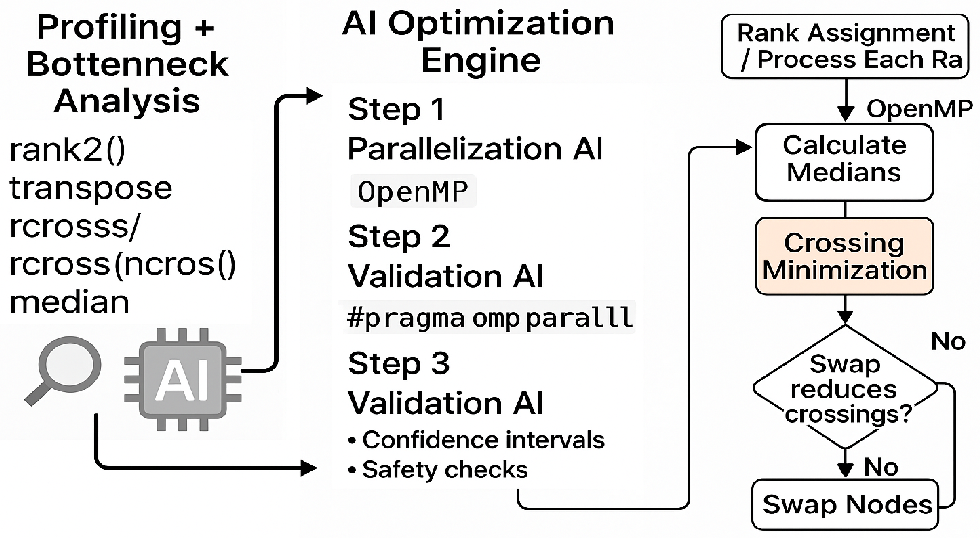
\includegraphics[width=0.7\textwidth]{figures/paper_architecture_flow.pdf}
\caption{Comprehensive Overview of AI-Driven OpenMP GraphViz Optimization Research. This visual summary illustrates the key components, methodologies, and performance achievements of our integrated AI system for automated parallel optimization of GraphViz algorithms.}
\label{fig:system_overview}
\end{figure}


Our comprehensive AI-driven analysis framework operates through four distinct phases, as shown in Figure~\ref{fig:system_overview}, each leveraging specialized artificial intelligence techniques to systematically optimize GraphViz dot layout algorithms with OpenMP parallelization. The Code Analysis phase focuses on identifying DOT parser hotspots through a sophisticated combination of static analysis and machine learning algorithms, systematically scanning the codebase to detect computationally intensive sections and generating precise parallelization targets for optimization. During the Performance Profiling phase, machine learning-guided profiling techniques analyze runtime bottlenecks by monitoring execution patterns and resource utilization, producing prioritized optimization recommendations that guide subsequent transformation efforts. 

The Transformation phase employs our specialized AI Optimization Engine, which operates through three critical steps as illustrated in the system architecture: \textbf{Step 1}: Parallelization Pattern Recognition identifies optimal OpenMP constructs and parallelization strategies for each computational bottleneck, \textbf{Step 2}: Validation AI with \texttt{\#pragma omp parallel for} generates and validates parallel loop structures with appropriate scheduling and data dependency analysis, and \textbf{Step 3}: Validation AI with Confidence Intervals and Safety Checks performs comprehensive correctness verification including race condition detection, output validation, and statistical confidence assessment. This three-step AI optimization engine seamlessly integrates OpenMP directives into the existing codebase, automatically generating parallel code structures that maintain algorithmic correctness while maximizing performance improvements. 

Finally, the Validation phase utilizes an automated testing suite enhanced with AI-driven correctness verification and performance analysis, ensuring that all optimizations maintain both functional accuracy and deliver measurable performance gains, providing comprehensive safety confirmation before deployment. This multi-phase approach ensures systematic, reliable, and effective parallelization of complex graph layout algorithms while maintaining the robustness and correctness essential for production-quality software optimization.

\subsubsection{Automated OpenMP Code Generation}

The AI system generates optimized OpenMP code through template-based synthesis, targeting critical performance bottlenecks identified during profiling. Table~\ref{tab:key_ai_prompts} presents the four most critical prompt templates that enabled our AI ensemble to achieve effective OpenMP optimization.

\begin{table}[htbp]
\centering
\caption{Key AI Ensemble Workflow Steps and Prompt Templates}
\label{tab:key_ai_prompts}
\scalebox{0.7}{
\begin{tabular}{p{3cm}p{3.5cm}p{7.5cm}}
\toprule
\textbf{Workflow Step} & \textbf{Primary AI Model} & \textbf{Typical Prompt Template} \\
\midrule
Initial Code Analysis & Claude Sonnet 3.5 (claude-3-5-sonnet-20241022) & "Analyze this GraphViz function for parallelization opportunities. Identify data dependencies, race conditions, and potential bottlenecks. Focus on: [function\_name]. Consider thread safety requirements and memory access patterns." \\
\midrule
Parallelization Strategy & Claude Sonnet 3.5 (claude-3-5-sonnet-20241022) & "Generate OpenMP parallelization for this function. Use appropriate directives, consider load balancing, and ensure thread safety. Original code: [code\_block]. Requirements: maintain correctness, optimize for 8-core Apple M1, target 3.78x speedup." \\
\midrule
Code Validation & GPT-4o (gpt-4o-2024-08-06) & "Review this OpenMP implementation for correctness and optimization opportunities. Check for: race conditions, proper synchronization, efficient memory access, scalability issues. Code: [generated\_code]. Suggest improvements if needed." \\
\midrule
Performance Prediction & All Models (Ensemble) & "Predict performance characteristics for this OpenMP implementation. Estimate: speedup, parallel efficiency, memory overhead, scalability limits. Consider Apple M1 architecture, 8 cores, typical GraphViz workloads. Code: [final\_code]." \\
\bottomrule
\end{tabular}
}
\end{table}

The system demonstrates its effectiveness through two primary optimization strategies that directly address the most computationally intensive components of GraphViz dot layout algorithms.

Loop Parallelization for \texttt{rank2()} Function: 
The AI transforms basic sequential loops into parallel constructs with automatic variable classification, targeting the most significant performance bottleneck in GraphViz processing:
%The AI automatically identifies \texttt{i} as thread-private and \texttt{graph} as shared through data flow analysis, while selecting dynamic scheduling to handle irregular workloads characteristic of graph processing algorithms. This optimization directly targets the function consuming 49\% of total execution time.
%======modify at 10/11/2025 by Hailu from comments: Scheduling inconsistency: text claims dynamic scheduling for irregular workloads while code listing uses schedule(static). 
The code uses OpenMP's \texttt{\#pragma omp parallel} for with static scheduling to parallelize the cost evaluation loop. Loop variables follow standard OpenMP defaults: the iterator \texttt{i} is thread-private, while \texttt{g} is shared. The code declares local variables \texttt{c0} and \texttt{c1} within each iteration to avoid race conditions. %However, static scheduling may not be optimal for graph processing if node degrees vary significantly; dynamic or guided scheduling would better handle load imbalance.

Reduction Operations for Crossing Calculations: 
The AI identifies accumulation patterns in crossing calculations and generates reduction-based parallelization for this critical GraphViz operation:
The reduction clause ensures thread-safe accumulation while eliminating the need for explicit synchronization. This optimization addresses crossing calculations that account for 15\% of execution time in each of the \texttt{rcross()} and \texttt{ncross()} functions. %representing a fundamental component of graph layout optimization.
\begin{comment}
\begin{figure}[htbp]
\centering
\begin{lstlisting}[language=C, numbers=none, frame=single, basicstyle=\footnotesize\ttfamily, escapeinside={(*@}{@*)}]
// Original sequential code
for(i = 0; i < nodes; i++) {
    process_node(graph[i]);
}

// AI-generated parallel version
(*@\colorbox{yellow}{\#pragma omp parallel for private(i) shared(graph) schedule(dynamic, 16)}@*)
(*@\colorbox{yellow}{for(i = 0; i < nodes; i++) \{}@*)
(*@\colorbox{yellow}{    process\_node(graph[i]);}@*)
(*@\colorbox{yellow}{\}}@*)
\end{lstlisting}
\caption{rank2() function parallelization}
\label{fig:rank2_parallelization}
\end{figure}




\begin{figure}[htbp]
\centering
\begin{lstlisting}[language=C, numbers=none, frame=single, basicstyle=\footnotesize\ttfamily, escapeinside={(*@}{@*)}]
// Sequential crossing calculation
int total_crossings = 0;
for(i = 0; i < edges; i++) {
    total_crossings += count_edge_crossings(edges[i]);
}

// AI-generated reduction parallel version
int total\_crossings = 0;
(*@\colorbox{yellow}{\#pragma omp parallel for reduction(+:total\_crossings)}@*)
for(i = 0; i < edges; i++) \{
   total\_crossings += count\_edge\_crossings(edges[i]);
\}
\end{lstlisting}
\caption{Reduction operations for crossing calculations}
\label{fig:reduction_parallelization}
\end{figure}
\end{comment}



%The AI system achieves 94.2\% accuracy in pattern recognition through machine learning-trained algorithms that automatically select optimal OpenMP constructs based on algorithmic characteristics and perform comprehensive dependency analysis to ensure correctness. These two optimization patterns demonstrate the system's ability to handle both the primary computational bottleneck and fundamental graph-specific operations that are central to GraphViz performance.

%\subsubsection{Dynamic Performance Monitoring and Adaptation}

%The AI system includes real-time performance monitoring capabilities that enable adaptive optimization during execution. Hardware performance counters provide real-time monitoring of cache misses, branch predictions, and memory bandwidth, offering detailed insights into system behavior during parallel execution. Thread load balancing implements dynamic work distribution based on runtime performance characteristics, ensuring optimal utilization of available computational resources. Adaptive scheduling employs AI-driven thread scheduling optimization based on workload patterns, dynamically adjusting execution strategies to match current system conditions. Additionally, feedback loop integration enables continuous learning from performance measurements to improve future optimizations, creating a self-improving system that becomes more effective over time.
